%%%%%%%%%%%%%%%%%%%%%%%%%%%%%%%%%%%%%%%%%
% a0poster Portrait Poster
% LaTeX Template
% Version 1.0 (22/06/13)
%
% The a0poster class was created by:
% Gerlinde Kettl and Matthias Weiser (tex@kettl.de)
% 
% This template has been downloaded from:
% http://www.LaTeXTemplates.com
%
% License:
% CC BY-NC-SA 3.0 (http://creativecommons.org/licenses/by-nc-sa/3.0/)
%
%%%%%%%%%%%%%%%%%%%%%%%%%%%%%%%%%%%%%%%%%

%----------------------------------------------------------------------------------------
%	PACKAGES AND OTHER DOCUMENT CONFIGURATIONS
%----------------------------------------------------------------------------------------

\documentclass[a0,portrait]{a0poster}

\usepackage{multicol} % This is so we can have multiple columns of text side-by-side
\columnsep=110pt % This is the amount of white space between the columns in the poster
\columnseprule=4pt % This is the thickness of the black line between the columns in the poster

\usepackage[svgnames]{xcolor} % Specify colors by their 'svgnames', for a full list of all colors available see here: http://www.latextemplates.com/svgnames-colors

%\usepackage{times} % Use the times font
\usepackage{palatino} % Uncomment to use the Palatino font

\usepackage{graphicx} % Required for including images
\graphicspath{{figures/}} % Location of the graphics files
\usepackage{booktabs} % Top and bottom rules for table
\usepackage[font=small,labelfont=bf]{caption} % Required for specifying captions to tables and figures
\usepackage{amsfonts, amsmath, amsthm, amssymb} % For math fonts, symbols and environments
\usepackage{wrapfig} % Allows wrapping text around tables and figures

% To be used on the tables
\usepackage{multirow} %
\usepackage{xcolor,colortbl}

\usepackage{titlesec}
\titleformat*{\section}{\Huge}
\titleformat*{\subsection}{\LARGE\bfseries}

\begin{document}

%----------------------------------------------------------------------------------------
%	POSTER HEADER 
%----------------------------------------------------------------------------------------

% The header is divided into two boxes:
% The first is 75% wide and houses the title, subtitle, names, university/organization and contact information
% The second is 25% wide and houses a logo for your university/organization or a photo of you
% The widths of these boxes can be easily edited to accommodate your content as you see fit

\begin{minipage}[b]{0.75\linewidth}
\veryHuge \color{NavyBlue} \textbf{TUW@Retrieving Diverse Social Images Task} \color{Black}\\ % Title
{\color{MediumAquamarine}
\Huge\textit{Working Notes}\\[2cm] % Subtitle
}
\huge \textbf{Joao Palotti* \& Navid Rekabsaz \& Mihai Lupu \& Allan Hanbury}\\[0.5cm] % Author(s)
\huge Vienna University of Technology\\[0.4cm] % University/organization
\Large \texttt{palotti@ifs.tuwien.ac.at} --- \color{NavyBlue} ifs.tuiwen.ac.at/$\sim$palotti \color{Black} \\
\end{minipage}
%
\begin{minipage}[b]{0.25\linewidth}

\includegraphics[width=20cm]{TU2.png}\\
\hspace{50cm} 
\includegraphics[width=12cm]{mucke.png}\\
\end{minipage}

\vspace{1cm} % A bit of extra whitespace between the header and poster content

%----------------------------------------------------------------------------------------

\begin{multicols}{2} % This is how many columns your poster will be broken into, a portrait poster is generally split into 2 columns

%----------------------------------------------------------------------------------------
%	OVERVIEW
%----------------------------------------------------------------------------------------

\large
\color{Navy} % Navy color for the abstract
\section*{Overview}

\begin{center}
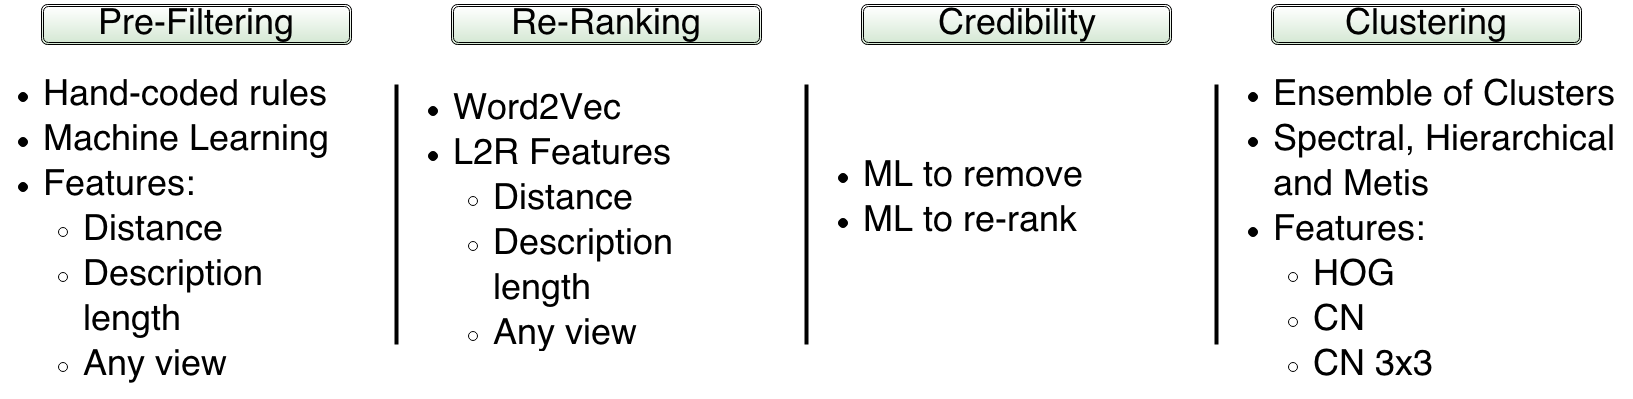
\includegraphics[width=1.05\linewidth]{overview_mediaeval}
\end{center}\vspace{0.5cm}

%----------------------------------------------------------------------------------------
%	INTRODUCTION
%----------------------------------------------------------------------------------------

\section*{Pre-filtering}
\large
\color{DarkSlateGray} % DarkSlateGray color for the rest of the content

We employed a pre-filtering step to exclude likely irrelevant pictures, increasing the percentage of relevant images.
We studied two approaches: 
\begin{enumerate}
\item Static rules to remove images without any view, geotagged more than 8 kilometers away from the point of interest (POI)
and with a description length longer than 2000 characters

\item Machine Learning (Logistic Regression classifier) on the whole 2013 and 2014 data, using as features the ones described
above and also the images' license, the time of the day (morning, afternoon, night) and the number of times the
POI appeared in the title and descriptions of an image 
\end{enumerate}


%----------------------------------------------------------------------------------------
%	RE-RANKING
%----------------------------------------------------------------------------------------


\color{Navy} % Navy color for the abstract
\section*{Re-ranking}
\color{DarkSlateGray} % DarkSlateGray color for the rest of the content

We tested four document similarity methods based on Solr, Random Indexing, Galago and Word2Vec.
The best performance was found using Word2Vec, which provides a vector representation of words by using deep learning.
We trained a model on Wikipedia and then used the vector representation of words to calculate the text similarity of the query to each photo.
Apart from the Word2Vec scores, we extracted binary attributes as we did in the pre-filtering
step, and we used a Linear Regression to re-rank the results based on the development data.

%For re-ordering the results, we used the title, tags and description of the photos. 
%For text pre-processing, we decomposed the terms using a greedy dictionary based approach.
%In the next step, we expand the query using the first sentence of Wikipedia which helped for place disambiguation.
%We tested four document similarity methods based on Solr, Random Indexing, Galago and Word2Vec. 
%Among all, we found the best result using a semantic similarity approach based on Word2Vec.
%Word2Vec provides vector representation of words by using deep learning. 
%We trained a model on Wikipedia and
%then used the vector representation of words to calculate
%the text similarity of the query to each photo.
%Apart from the Word2Vec scores, we extracted binary attributes based on Jain et al. [2], as we did in the pre-filtering
%step, and we used a Linear Regression to re-rank the results based on the development data.

%----------------------------------------------------------------------------------------
%	CREDIBILITY
%----------------------------------------------------------------------------------------

\color{Navy} % Navy color for the abstract
\section*{Credibility}
\color{DarkSlateGray} % DarkSlateGray color for the rest of the content

Our approaches were based on Machine Learning (ML):
we trained a Logistic Regression classifier to learn if a document was relevant or not based on the credibility data (used
only face proportion, location similarity, upload frequency
and bulk proportion). We tested two methods: (1) excluding documents set as irrelevant for Run4 and (2) moving to
the bottom of the list irrelevant documents for Run5.
%------------------------------------------------

%%%% COL 2

%----------------------------------------------------------------------------------------
%	CLUSTERING
%----------------------------------------------------------------------------------------
\color{Navy} % Navy color for the abstract
\section*{Clustering}
\color{DarkSlateGray} % DarkSlateGray color for the rest of the content

We worked on three methods for clustering, all based on similarity measures.
They share the idea of creating a similarity graph (potentially complete) in which each vertex represents an image for one point of interest, and
each edge represents the similarity between two images. Different similarity metrics and different set of features can be used.

\vspace{-0.4cm}
\subsection*{Metis}
\vspace{-0.8cm}

The method called Metis tries to collapse similar and neighbor vertices, reducing the initial graph to a smaller one (coarsening step).
Then, it divides the coarsest graph into a pre-defined number of graphs, creating the clusters.  

\vspace{-0.4cm}
\subsection*{Spectral}
\vspace{-0.8cm}

Spectral clustering can also be seen as a graph partitioning method, which measures both the total dissimilarity between groups 
as well as the total similarity within a group. %We used the Scikit-learn implementation of this method. 

\vspace{-0.4cm}
\subsection*{Hierarchical}
\vspace{-0.7cm}

Hierarchical clustering  is based on the idea of a hierarchy of clusters. A tree is built in a way that the root gathers all the samples and the leaves are clusters with only one sample. This tree can be built bottom-up or top-down. We used the bottom-up implementation from Scikit-learn.

\vspace{-0.4cm}
\subsection*{Ensembling}
\vspace{-0.7cm}

We found that the clustering methods were unstable as modifications in the filtering step caused a great variation in the clustering step.
Therefore, we decided to implement a merging heuristic, which takes into account different points of view from each clustering method and/or feature set,
being potentially more robust than using one single algorithm.

%Given $c$ different clustering algorithms, $f$ different feature sets, and $m$ distance measures, there are $c \times f \times m$ possible cluster sets. 
%In our work, we used the 3 algorithms described, 3 features sets (HOG, CN, CN3x3, see \cite{overview14} for details about these features) and 2 distance measures (cosine and Chebyshev), giving us 18 different cluster sets for each POI.
%We can then compute a \emph{frequency matrix} that will hold for every two documents the number of cluster sets in which they occur in the same cluster.
%Next we create a re-ranked list of the images from the original list (Flickr ranking) based only on this frequency matrix.
%In order to do that, we define a threshold $t$ and a function $F$ on a set of frequencies that determine when a document should be moved to the re-ranked list.
%Suppose the re-ranked list contains the documents $D_1, ..., D_i$ and we want to know if a document $D_k$ in the original list can be moved to the re-ranked list at position $i+1$. We compute the frequencies $f_1, ..., f_i$ between $D_k$ and each $D_1,...,D_i$ and if $F(f_1, ..., f_i) < t$, $D_k$ is moved to the re-ranked list, otherwise it is not. 
%After all the elements in the original list are processed, if there are still remaining documents not moved to the re-ranked list, the value of $t$ is increased and these documents are reprocessed. The algorithm continues until there are no documents left in the original list.
%The functions for $F$ used in this work were maximum, minimum and mean, but other measures, such as mode, median or any percentile could be easily employed as well.

We consider that each clustering algorithm can be used with different sets of features and similarity measures: \textbf{Cluster}(\textit{Algorithm, Distance Metric, Feature Set}).
The main measure used for re-ranking the original list is the frequency that two images are set to the same cluster in the ensemble.


\begin{center}\vspace{0.5cm}
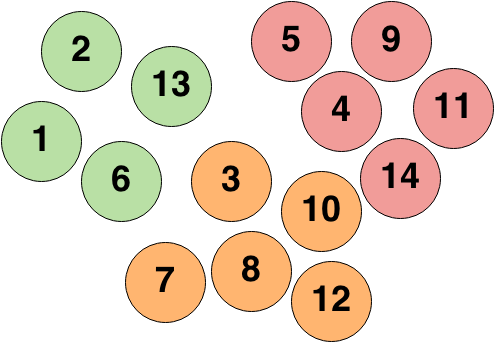
\includegraphics[width=.3\linewidth]{cluster1.png} ~
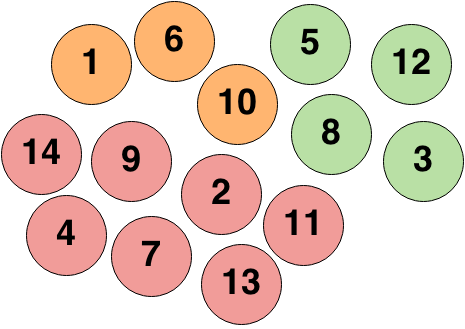
\includegraphics[width=.3\linewidth]{cluster2.png} ~
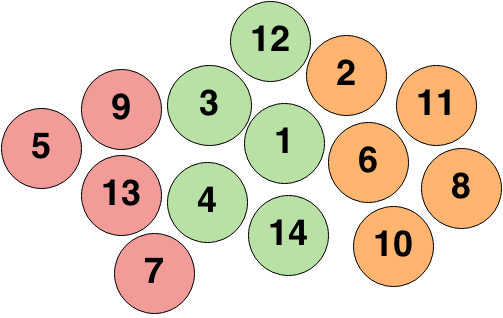
\includegraphics[width=.3\linewidth]{cluster3.png}
\captionof{figure}{\color{Green} \normalsize Three different ways to cluster 14 images. Different clustering algorithms, similarity measures and feature sets can strongly change the clustering assignments}
\end{center}%\vspace{0.5cm}

\begin{center}%\vspace{0.5cm}
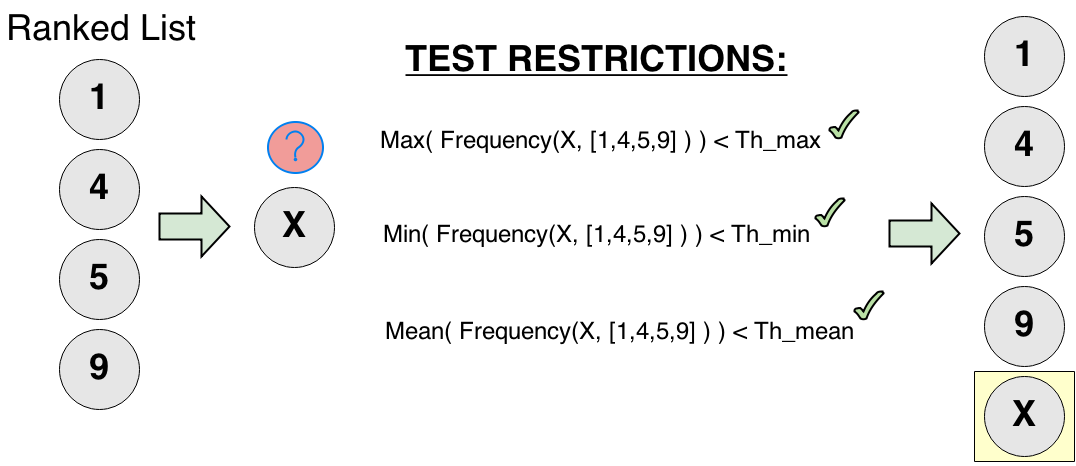
\includegraphics[width=0.8\linewidth]{poster.png} 
\captionof{figure}{\color{Green} \normalsize Illustrates how simple frequency-based rules can be effectively used to decide if an element should be added to the final re-ranked list.}
\end{center} %\vspace{0.5cm}


%----------------------------------------------------------------------------------------
%	RESULTS 
%----------------------------------------------------------------------------------------

\color{Navy} % Navy color for the abstract
\section*{Results}
\color{DarkSlateGray} % DarkSlateGray color for the rest of the content

The configuration of our 5 runs and their results were:
\begin{center} %\vspace{1cm}
\label{table:config}
\normalsize
\begin{tabular}{c|c|c|c|c}
\toprule 
\textbf{Run} & \textbf{Pre-Filtering} & \textbf{Re-Ranking}  & \textbf{Credibility} & \textbf{Clustering}\tabularnewline
\midrule
\textbf{1} & Static Rules & - & - & Combined on HOG,CN3x3,CN \tabularnewline
\textbf{2} & - & Word2Vec & - & Metis on Text Similarity \tabularnewline
\textbf{3} & - & Word2Vec & - & Combined on HOG,CN3x3,CN \tabularnewline
\textbf{4} & - & Word2Vec &   ML to remove elements & Combined on HOG,CN3x3,CN\tabularnewline
\textbf{5} & Based on ML & Word2Vec  & ML to re-rank elements & Combined on HOG,CN3x3,CN\tabularnewline
\bottomrule 
\end{tabular}
\end{center} %\vspace{1cm}

\vspace{1cm}
Run 1 was the best one, reaching a F@20 of 0.56.
\begin{center}
\normalsize
\begin{tabular}{c||c|c|c|c|c|c||c|c|c|c|c|c}
\toprule 
\multirow{2}{*}{\textbf{Run}} & \multicolumn{6}{c||}{\textbf{2014 Development Set}} & \multicolumn{6}{c}{\textbf{2014 Test Set}}\tabularnewline
\cmidrule{2-13} 
 & \textbf{P@10} & \textbf{CR@10} & \textbf{F1@10} & \textbf{P@20} & \textbf{CR@20} & \textbf{F@20} & \textbf{P@10} & \textbf{CR@10} & \textbf{F1@10} & \textbf{P@20} & \textbf{CR@20} & \textbf{F@20}\tabularnewline
\midrule
\rowcolor{LightCyan}
\textbf{1} & 0.827 & 0.282 & 0.416 & 0.805 & 0.465 & 0.585 & 0.798 & \textbf{0.283}  & \textbf{0.412}  & 0.769  & \textbf{0.450}  & \textbf{0.560} \tabularnewline
\textbf{2} & \textbf{0.903} & 0.262 & 0.400 & \textbf{0.870} & 0.425 & 0.564 & \textbf{0.806} & 0.251  & 0.377  & \textbf{0.773}  & 0.381  & 0.501 \tabularnewline
\textbf{3} & 0.870 & \textbf{0.301} & \textbf{0.444} & 0.813 & 0.483 & 0.601 & 0.794 & 0.281  & 0.410  & 0.744  & 0.449  & 0.553 \tabularnewline
\textbf{4} & 0.890 & 0.297 & 0.441 & 0.827 & \textbf{0.503} & \textbf{0.619} & \textbf{0.806} & 0.280 & \textbf{0.412} & 0.754  & 0.443 &  0.552   \tabularnewline
\textbf{5} & 0.837 & 0.299 & 0.435 & 0.792 & 0.478 & 0.588 & 0.780 & 0.276 & 0.403 & 0.729 & 0.444 &  0.546    \tabularnewline
\bottomrule 
\end{tabular}
\end{center}\vspace{1cm}

%----------------------------------------------------------------------------------------
%	CONCLUSIONS
%----------------------------------------------------------------------------------------


\color{Navy} % Navy color for the abstract
\section*{Conclusions}
\color{DarkSlateGray} % DarkSlateGray color for the rest of the content

\begin{itemize}
\item Ensemble of clusters is a simple and very robust way to diversify results.
\item Few data for Machine Learning methods may be the main reason for overfiting the development set (and not improving for Runs 2,3,4 and 5) 
\item Future: evaluate the clustering procedure in other scenarios (e.g., text).
\end{itemize}


%----------------------------------------------------------------------------------------
%	FORTHCOMING RESEARCH
%----------------------------------------------------------------------------------------

%\color{Navy} % Navy color for the abstract
%\section*{Forthcoming Research}
%\color{DarkSlateGray} % DarkSlateGray color for the rest of the content

%Vivamus molestie, risus tempor vehicula mattis, libero arcu volutpat purus, sed blandit sem nibh eget turpis. Maecenas rutrum dui blandit lorem vulputate gravida. Praesent venenatis mi vel lorem tempor at varius diam sagittis. Nam eu leo id turpis interdum luctus a sed augue. Nam tellus.

%----------------------------------------------------------------------------------------
%	REFERENCES
%----------------------------------------------------------------------------------------

%\nocite{*} % Print all references regardless of whether they were cited in the poster or not
%\bibliographystyle{plain} % Plain referencing style
%\bibliography{sample} % Use the example bibliography file sample.bib

%----------------------------------------------------------------------------------------
%	ACKNOWLEDGEMENTS
%----------------------------------------------------------------------------------------

\color{Navy} % Navy color for the abstract
\section*{Acknowledgements}

\color{SaddleBrown} % SaddleBrown color for the conclusions to make them stand out
This research was funded by the Austrian Science Fund (FWF) project number I1094-N23 (MUCKE) and project number P25905-N23 (ADmIRE). 
The authors would like also to thank the organizers for their excellent work.

\color{DarkSlateGray} % Set the color back to DarkSlateGray for the rest of the content
%----------------------------------------------------------------------------------------

\end{multicols}
\end{document}
